\documentclass[12pt,a4paper]{report}

\usepackage[utf8]{inputenc}
\usepackage[spanish]{babel}
\usepackage{graphicx}
\usepackage{amsmath}
\usepackage{amssymb}
\usepackage{hyperref}
\usepackage{geometry}
\usepackage{caption}
\usepackage{subcaption}
\geometry{a4paper, margin=1in}

\title{Segmentación Multimodal para detección de Animales}
\author{
    Jorge Urbón Burgos \\
    \texttt{777295@unizar.es}
    \and
    Supervisor: Rosario Aragües \\
    \texttt{raragues@unizar.es}
    \and
    Co-Supervisor: Jesús Bermúdez \\
    \texttt{bermudez@unizar.es}
}
\date{\today}

\begin{document}

\maketitle

\begin{abstract}
% TODO: add abstract
\end{abstract}

\tableofcontents

\chapter{Introduction}
\label{chap:introduction}
Image segmentation has been a fundamental problem in computer vision tasks since the early days of the field. The main goal of image segmentation is to partition an image into multiple regions or objects

\chapter{Literature Review}
\label{chap:literature_review}
% TODO: add literature review

\chapter{Metodología}
\label{chap:methodology}
\section{Data}
\label{sec:data}
\subsection{Lindenthal Dataset}
\label{subsec:lindenthal_dataset}
\subsection{Técnicas de Post Procesado}
\label{subsec:tecnicas_post_procesado}
Existe una variedad de técnicas de post-procesado que aprovechan los tres canales de entrada del modelo para así lograr un \textit{input} capaz de aportar mayor cantidad de información al modelo de segmentación. Además, al consistir el \textit{dataset} en imágenes obtenidas con una cámara estéreo \texttt{Intel RealSense D435}, la cantidad de ruido en las imágenes es considerable, por lo que toda técnica que ayude a destacar los objetos de interés será importante para el correcto desempeño del modelo.

\subsubsection{Equalización del Histograma}
La primera técnica de postprocesado a implementar consiste en la equalización del histograma de valores en la imagen. Esto puede suponer una gran mejora en la forma en la que se representan las imágenes debido a que no todo el rango de valores de intensidad es aprovechado dado a que la mayoría de los objetos de interés se encuentran a una distancia relativamente baja de la cámara. Equalizar el histograma puede permitir destacar ciertos objetos que de otra forma no serían tan visibles.
\begin{figure}[!h]
    \centering
    \begin{subfigure}{0.45\textwidth}
        \centering
        
\includegraphics[width=\textwidth]{media/data/depth_gueese.png}
        \caption{Imagen de profundidad base}
    \end{subfigure}
    \hfill
    \begin{subfigure}{0.45\textwidth}
        \centering
        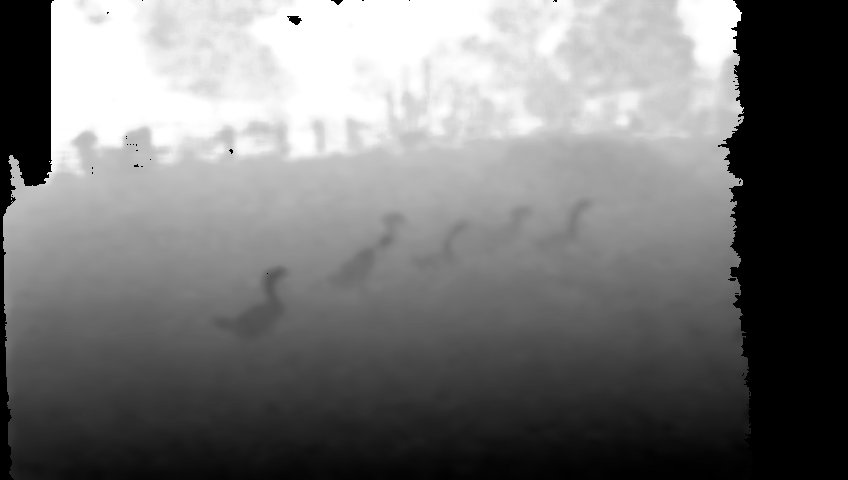
\includegraphics[width=\textwidth]{media/data/deptheq_gueese.png}
        \caption{Histograma equalizado}
    \end{subfigure}
    \caption{Comparación entre la imagen de profundidad base y la imagen con el histograma equalizado}
    \label{fig:depth-histeq-comparison}
\end{figure}
Como se puede observar en la figura \ref{fig:histogram-comparison}, la ecualización del histograma permite un mayor reparto de los valores de intensidad en la imagen, lo que aprovecha aquellos rangos menos utilizados en la imagen original permitiendo así un mayor contraste entre los rangos más utilizados en la imagen original como se puede observar en la figura \ref{fig:depth-histeq-comparison}.
Esta técnica, sin embargo, puede no ser adecuada para otras aplicaciones, ya que se pierde la información real sobre la distancia de los objetos a la cámara.
\begin{figure}[!h]
    \centering
    \begin{subfigure}{0.45\textwidth}
        \centering
        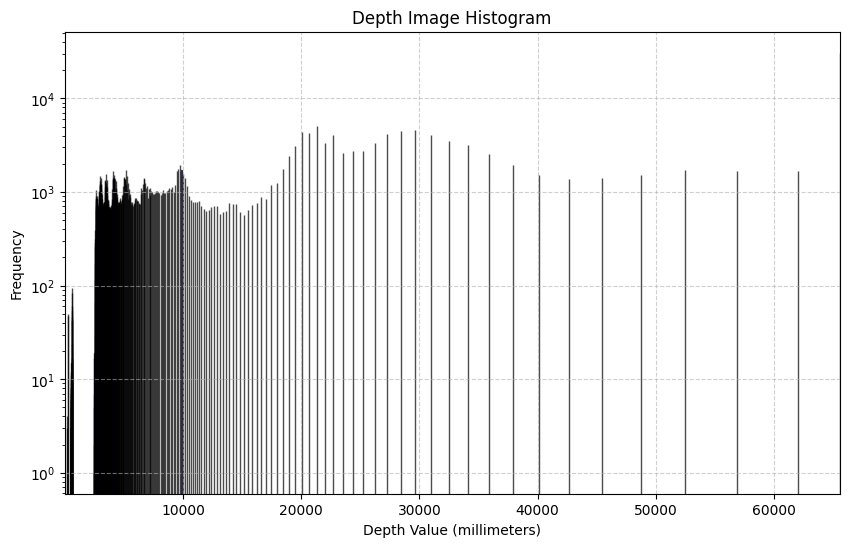
\includegraphics[width=\textwidth]{media/data/normal_histogram.png}
        \caption{Histograma de la imagen de profundidad base}
    \end{subfigure}
    \hfill
    \begin{subfigure}{0.45\textwidth}
        \centering
        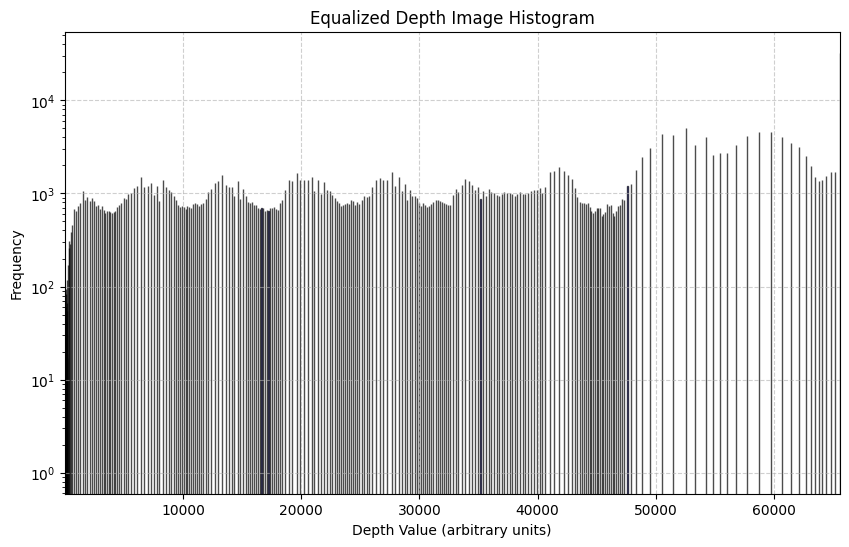
\includegraphics[width=\textwidth]{media/data/equalized_histogram.png}
        \caption{Histograma de la imagen con el histograma equalizado}
    \end{subfigure}
    \caption{Comparación entre los histogramas de la imagen de profundidad base y la imagen con el histograma equalizado}
    \label{fig:histogram-comparison}
\end{figure}

\subsubsection{HHA Encoding}
\label{subsubsec:hha_encoding}
Esta técnica, propuesta por \cite{gupta2014learningrichfeaturesrgbd} usa los tres canales de la imagen de entrada para codificar las siguientes tres características:
\begin{itemize}
    \item Altura sobre el suelo
    \item Disparidad horizontal
    \item Ángulo con respecto a la gravedad
\end{itemize}
Estas colorización, además de implementar características que difícilmente serían aprendidas por el modelo si no se codificaran en la imagen de entrada, aprovecha los tres canales de entrada al \textit{encoder}, por lo que los pesos ya preentrenados en \textit{ImageNet} pueden ser empleados para una mejor comprensión de la escena.
\begin{figure}[!h]
    \centering
    \begin{subfigure}{0.45\textwidth}
        \centering
        
\includegraphics[width=\textwidth]{media/data/depth_gueese.png}
        \caption{Imagen de profundidad base}
    \end{subfigure}
    \hfill
    \begin{subfigure}{0.45\textwidth}
        \centering
        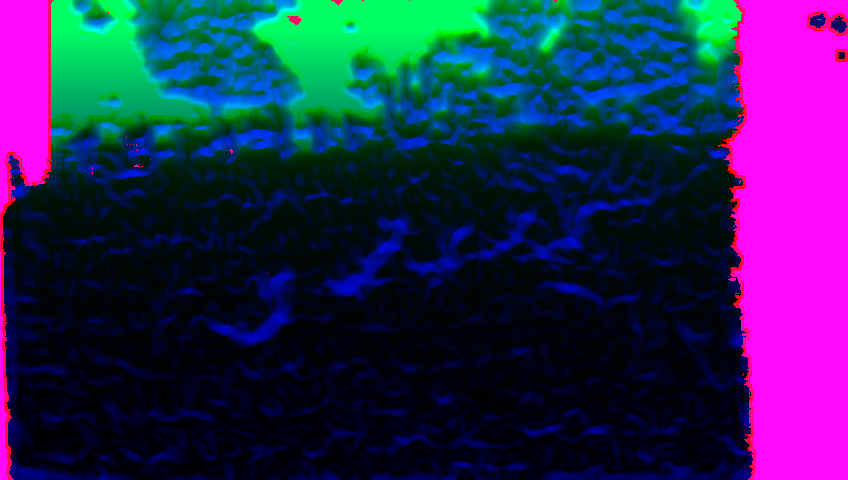
\includegraphics[width=\textwidth]{media/data/hha_gueese.png}
        \caption{Profundidad colorizada con HHA}
    \end{subfigure}
    \caption{Comparison between the base depth image and the HHA encoded image}
    \label{fig:depth-hha-comparison}
\end{figure}

\subsubsection{Colorizacón Jet}
\label{subsubsec:jet_colorization}
Otra posible técnica es la colorización de la imagen de entrada usando el esquema de color \textit{Jet} mostrado en la figura \ref{fig:jet-colormap}, lo que implica la asignación de un valor \textit{RGB} a cada píxel dependiendo de su valor de intensidad. Esto, de forma similar a \ref{subsubsec:hha_encoding}, permite al modelo aprovechar sus pesos ya entrenados en \textit{ImageNet} para identificar con mayor facilidad los objetos a segmentar.
\begin{figure}[!h]
    \centering
    
\includegraphics[width=0.5\textwidth]{media/misc/jet_colormap.png}
    \caption{\textit{Jet} colormap}
    \label{fig:jet-colormap}
\end{figure}
\begin{figure}[!h]
    \centering
    \begin{subfigure}{0.45\textwidth}
        \centering
        
\includegraphics[width=\textwidth]{media/data/depth_gueese.png}
        \caption{Imagen de profundidad base}
    \end{subfigure}
    \hfill
    \begin{subfigure}{0.45\textwidth}
        \centering
        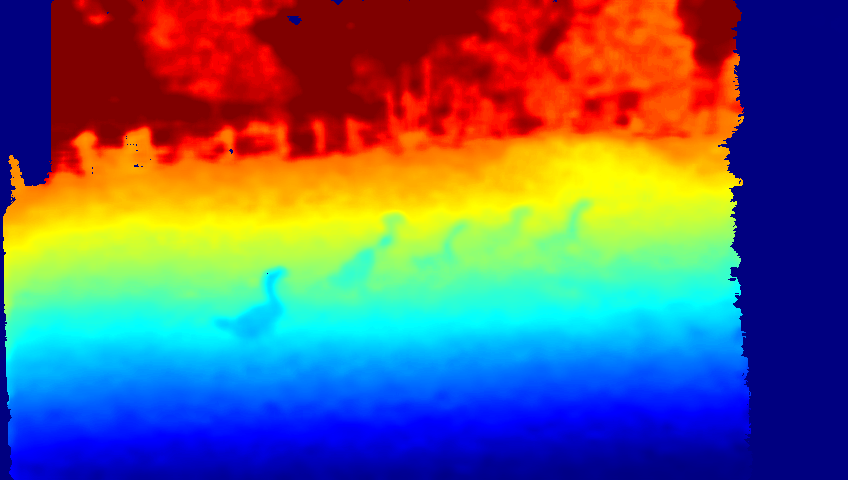
\includegraphics[width=\textwidth]{media/data/jet_gueese.png}
        \caption{Profundidad colorizada con \textit{Jet}}
    \end{subfigure}
    \caption{Comparación entre la imagen de profundidad y la colorización \textit{Jet}}
    \label{fig:depth-jet-comparison}
\end{figure}

\subsubsection{Normales}
\label{subsubsec:normals}
La última técnica de postprocesado a implementar consiste en la codificación de las normales en la imagen de entrada. Esta técnica consiste en calcular el vector normal de la superficie de cada pixel partiendo de la imagen de profundidad y codificarlo en los tres canales del \textit{input} del modelo. Esto permite al modelo aprender características de la escena que de otra forma serían difíciles de aprender, como la orientación de los objetos en la escena.
\begin{figure}[!h]
    \centering
    \begin{subfigure}{0.45\textwidth}
        \centering
        
\includegraphics[width=\textwidth]{media/data/depth_gueese.png}
        \caption{Imagen de profundidad base}
    \end{subfigure}
    \hfill
    \begin{subfigure}{0.45\textwidth}
        \centering
        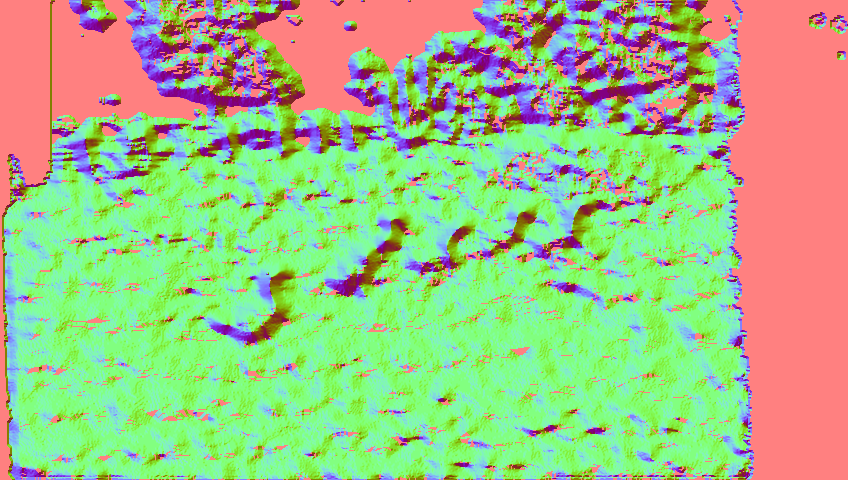
\includegraphics[width=\textwidth]{media/data/normal_gueese.png}
        \caption{Normales codificadas en la imagen de profundidad}
    \end{subfigure}
    \caption{Comparación entre la imagen de profundidad y la codificación de las normales}
    \label{fig:depth-normals-comparison}
\end{figure}

\subsubsection{Comparación de Técnicas}
\label{subsubsec:techniques_comparison}
Las distintas técnicas anteriores presentan diferentes resultados a la hora de ser aplicadas al \textit{input} del modelo. La tabla \ref{tab:techniques-comparison} muestra una comparación entre las distintas técnicas de postprocesado.
\begin{table}[!h]
    \centering
    \begin{tabular}{|c|c|c|c|c|}
        \hline
        Técnica & Equalización & HHA & Jet & Normales \\
        \hline
        \hline
        Deer IoU & 0.000 & 0.000 & 0.000 & 0.000 \\
        \hline
        Goat IoU & 0.000 & 0.000 & 0.000 & 0.000 \\
        \hline
        Donkey IoU & 0.000 & 0.000 & 0.000 & 0.000 \\
        \hline
        Goose IoU & 0.000 & 0.000 & 0.000 & 0.000 \\
        \hline
        \textbf{Mean} IoU & 0.000 & 0.000 & 0.000 & 0.000 \\
        \hline
    \end{tabular}
    \caption{Comparación entre las distintas técnicas de postprocesado}
    \label{tab:techniques-comparison}
\end{table}

\chapter{Results}
\label{chap:results}
% TODO: add results

\chapter{Discussion}
\label{chap:discussion}
% TODO: add discussion

\chapter{Conclusion}
\label{chap:conclusion}
% TODO: add conclusion and future work

\bibliography{refs.bib}
\bibliographystyle{IEEEtran}

\appendix
\label{app:appendix_a}
% TODO: whatever appendices :)

\end{document}